
Given a basis $\mathcal A$ for $\R^n$, every  vector $\vec x\in\R^n$ uniquely
corresponds to the list of numbers $[\vec x]_{\mathcal A}$ (its coordinates with respect
to $\mathcal A$), and  the operation of writing a vector in a basis is \emph{invertible}.

If we have two bases, $\mathcal A$ and $\mathcal B$, for $\R^n$, we have two equally valid
ways of representing a vector in coordinates.

\begin{center}
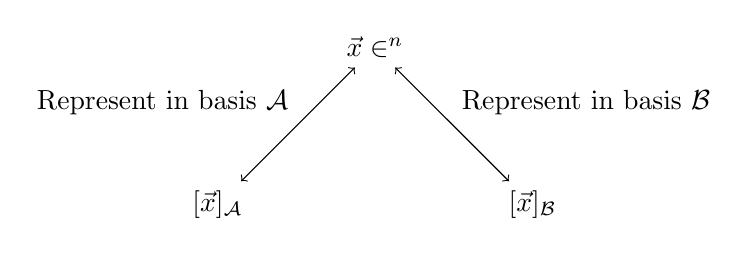
\begin{tikzpicture}
	\node (A) at (0,0) {$\vec x\in \R^n$};
	\node (B) at (-2,-2) {$[\vec x]_{\mathcal A}$};
	\node (C) at (2,-2) {$[\vec x]_{\mathcal B}$};
	\draw[<->] 
		(A) edge  node[midway, above left] {Represent in basis $\mathcal{A}$}(B)
		(A) edge  node[midway, above right] {Represent in basis $\mathcal{B}$} (C);
\end{tikzpicture}
\end{center}

Not only that, but there must be a function that converts between $[\vec x]_{\mathcal A}$ and $[\vec x]_{\mathcal B}$.
The function works as follows: input the list of numbers $[\vec x]_{\mathcal A}$, use
those numbers as coefficients of the $\mathcal A$ basis vectors to get the true vector $\vec x$, and then find
the coordinates of that vector with respect to the $\mathcal B$ basis.

\begin{example}
	Let $\mathcal A=\Set{\vec a_1,\vec a_2}$ where $\vec a_1=\mat{1\\1}_{\mathcal E}$ and $\vec a_2=\mat{1\\-1}_{\mathcal E}$ and let
	$\mathcal B=\Set{\vec b_1,\vec b_2}$ where $\vec b_1=\mat{2\\1}_{\mathcal E}$ and $\vec b_2=\mat{5\\3}_{\mathcal E}$ be bases for $\R^2$.
	Given that $[\vec x]_{\mathcal A}=\mat{2\\-3}$, find $[\vec x]_{\mathcal B}$.

	By definition,
	\[
		\vec x=2\vec a_1-3\vec a_2=2(\xhat+\yhat)-3(\xhat-\yhat)=-\xhat+5\yhat.
	\]
	We need to rewrite $\vec x$ as a linear combination of $\vec b_1=2\xhat+\yhat$ and $\vec b_2=5\xhat+3\yhat$. That is,
	we need to solve the equation
	\[
		\vec x=-\xhat+5\yhat = \alpha(2\xhat+\yhat)+\beta(5\xhat+3\yhat)=(2\alpha+5\beta)\xhat+(\alpha+3\beta)\yhat.
	\]
	Equating the coefficients of $\xhat$ and $\yhat$, we get
	\[
		\systeme[\alpha\beta]{2\alpha+5\beta=-1,\alpha+3\beta=5},
	\]
	which has a unique solution $(\alpha,\beta)=(-28,11)$. We conclude
	\[
		[\vec x]_{\mathcal B} =\mat{-28\\11}.
	\]
\end{example}

For a basis $\mathcal A$, the invertible function that takes a vector $\vec x$ and generates the coordinates $[\vec x]_{\mathcal A}$
is a linear function. Therefore, for bases $\mathcal A$ and $\mathcal B$, the function that converts $[\vec x]_{\mathcal A}$ to $[\vec x]_{\mathcal B}$
must have a matrix. This matrix is called the \emph{change of basis} matrix.

\SavedDefinitionRender{ChangeofBasisMatrix}

\begin{example}
	Let $\mathcal A=\Set{\vec a_1,\vec a_2}$ where $\vec a_1=\mat{1\\1}_{\mathcal E}$ and $\vec a_2=\mat{1\\-1}_{\mathcal E}$ and let
	$\mathcal B=\Set{\vec b_1,\vec b_2}$ where $\vec b_1=\mat{2\\1}_{\mathcal E}$ and $\vec b_2=\mat{5\\3}_{\mathcal E}$ be bases for $\R^2$.
	Find the change of basis matrix $\BasisChange{\mathcal A}{\mathcal B}$.

	We know $\BasisChange{\mathcal A}{\mathcal B}$ will be a $2\times 2$ matrix and that
	\[
		\BasisChange{\mathcal A}{\mathcal B}[\vec a_1]_{\mathcal A}=[\vec a_1]_{\mathcal B}\qquad
		\text{and}\qquad
		\BasisChange{\mathcal A}{\mathcal B}[\vec a_2]_{\mathcal A}=[\vec a_2]_{\mathcal B}.
	\]
	Therefore, we need to compute $[\vec a_1]_{\mathcal B}$ and $[\vec a_2]_{\mathcal B}$. Repeating the procedure from the previous example,
	we find
	\[
		[\vec a_1]_{\mathcal B}=\mat{-2\\1}\qquad \text{and}\qquad [\vec a_2]_{\mathcal B}=\mat{8\\-3},
	\]
	and so
	\[
		\BasisChange{\mathcal A}{\mathcal B}=\mat{-2&8\\1&-3}.
	\]
\end{example}

We can now enhance our diagram from earlier.

\begin{center}
\begin{tikzpicture}
	\node (A) at (0,0) {$\vec x\in \R^n$};
	\node (B) at (-2,-2) {$[\vec x]_{\mathcal A}$};
	\node (C) at (2,-2) {$[\vec x]_{\mathcal B}$};
	\draw[<->] 
		(A) edge  node[midway, above left] {Represent in $\mathcal{A}$ basis}(B)
		(A) edge  node[midway, above right] {Represent in $\mathcal{B}$ basis} (C);
	\draw[->, dashed, transform canvas={yshift=-.25em}, mygreen] 
		(B) edge  node[midway, below] {$\BasisChange{\mathcal A}{\mathcal B}$} (C);
	\draw[<-, dashed, transform canvas={yshift=.25em}, mypink] 
		(B) edge  node[midway, above] {$\BasisChange{\mathcal B}{\mathcal A}$} (C);
\end{tikzpicture}
\end{center}

The notation $\BasisChange{\mathcal A}{\mathcal B}$ for the matrix that changes from the $\mathcal A$ basis to
the $\mathcal B$ basis is suggestive. Suppose we have another basis $\mathcal C$. We can obtain
$\BasisChange{\mathcal A}{\mathcal C}$ by multiplying $\BasisChange{\mathcal A}{\mathcal B}$ on the left by $\BasisChange{\mathcal B}{\mathcal C}$.
That is,
\[
	\BasisChange{\mathcal A}{\mathcal C}=\BasisChange{\mathcal B}{\mathcal C}\BasisChange{\mathcal A}{\mathcal B}.
\]
The backwards arrow ``$\leftarrow$'' in the change-of-basis matrix notation comes because when we multiply a
vector and a matrix, the matrix is always to the \emph{left} of the vector. So, \[
	[\vec x]_{\mathcal C}=
	\BasisChange{\mathcal A}{\mathcal C}[\vec x]_{\mathcal A}
	=\BasisChange{\mathcal B}{\mathcal C}\BasisChange{\mathcal A}{\mathcal B}[\vec x]_{\mathcal A}.
\]
As such, the notation for the change of basis matrix chains, allowing you to figure out what's going on without too much trouble.

\Heading{Change of Basis Matrix in Detail}

Let $\mathcal A$ and $\mathcal B$ be bases for $\R^n$ and $M=\BasisChange{\mathcal A}{\mathcal B}$ be the matrix
that changes from the $\mathcal A$ to the $\mathcal B$ basis. Since we can change vectors back from $\mathcal B$ to
$\mathcal A$, we know $M$ is invertible and
\[
	M^{-1}=\BasisChange{\mathcal B}{\mathcal A}.
\]
Just playing with notation, we see
\[
	M^{-1}M=\BasisChange{\mathcal B}{\mathcal A}\BasisChange{\mathcal A}{\mathcal B}=\BasisChange{\mathcal A}{\mathcal A} = I\qquad
	MM^{-1}=\BasisChange{\mathcal A}{\mathcal B}\BasisChange{\mathcal B}{\mathcal A}=\BasisChange{\mathcal B}{\mathcal B} = I,
\]
which makes sense. The matrices $\BasisChange{\mathcal A}{\mathcal A}$ and $\BasisChange{\mathcal B}{\mathcal B}$
take vectors and rewrite them in the same basis, which is to say, they do nothing to the vectors.

The argument above shows that every change of basis matrix is invertible. The converse is also true.

\begin{theorem}
	An $n\times n$ matrix is invertible\index{Matrix!invertible} if and only if it is a change of basis matrix.
\end{theorem}
\begin{proof}
	Suppose $M=\BasisChange{\mathcal A}{\mathcal B}$ is a change-of-basis matrix. Then
	\[
		M^{-1}=\BasisChange{\mathcal B}{\mathcal A},
	\]
	and so $M$ is invertible.

	Alternatively, suppose $M=[C_1|C_2|\cdots|C_n]$ is an invertible $n\times n$ matrix with columns $C_1$, \ldots, $C_n$.
	Let $\vec c_i=[C_i]_{\mathcal E}$. That is, $\vec c_i$ is the vector which comes from interpreting $C_i$ as coordinates
	with respect to the standard basis.

	Since $M$ is invertible, $\Rref(M)=I$, and so $\Set{\vec c_1,\ldots,\vec c_n}$ is a linearly independent set of $n$ vectors.
	Therefore $\mathcal C=\Set{\vec c_1,\ldots,\vec c_n}$ is a basis for $\R^n$. Now, observe
	\[
		M[\vec c_i]_{\mathcal C} = C_i=[\vec c_i]_{\mathcal E}
	\]
	for $i=1,\ldots, n$,
	and so $M=\BasisChange{\mathcal C}{\mathcal E}$ is a change-of-basis matrix.
\end{proof}

The proof of the above theorem highlights something interesting. Let $\mathcal A=\Set{\vec a_1,\ldots, \vec a_n}$
be a basis for $\R^n$. It is always the case that
\[
	[\vec a_i]_{\mathcal A}=\matc{\vdots\\0\\1\\0\\0\\\vdots}
\]
has a $1$ in the $i$th position and zeros elsewhere. Now, let 
$\mathcal B=\Set{\vec b_1,\ldots,\vec b_n}$ be another basis for $\R^n$
and define the matrix $M=\mat{[\vec a_1]_{\mathcal B}&[\vec a_2]_{\mathcal B}&\cdots&[\vec a_n]_{\mathcal B}}$
to be the matrix with columns $[\vec a_1]_{\mathcal B},\ldots, [\vec a_n]_{\mathcal B}$.
Since multiplying a matrix by $[\vec a_i]_{\mathcal A}$ will pick out the $i$th column, we have that
\[
	M[\vec a_i]_{\mathcal A} = [\vec a_i]_{\mathcal B}.
\]
In other words,
\[
	M=\BasisChange{\mathcal A}{\mathcal B}.
\]

\Heading{Transformations and Bases}
A linear transformation $\mathcal T:\R^n\to\R^n$ always has a matrix associated with it.
This matrix is defined as the matrix $M$ so that
\[
	[\mathcal T\vec x]_{\mathcal E}=M[\vec x]_{\mathcal E}.
\]
But, what if we swapped out $\mathcal E$ for a different basis?

\SavedDefinitionRender{LinearTransformationinaBasis}

Just like there are many ways to write down coordinates for a vector---one per choice of basis---there
are many ways to write down a matrix for a linear transformation. Up to this point, when we've said
``$M$ is a matrix for $\mathcal T$'', what we meant is ``$M=[\mathcal T]_{\mathcal E}$''. And, like
with vectors, if we talk about a matrix for a linear transformation without specifying the basis,
we mean the matrix for the transformation with respect to the standard basis.

\begin{example}
	Let $\mathcal B=\Set{\vec b_1,\vec b_2}$ where $\vec b_1=\mat{2\\-3}_{\mathcal E}$ and $\vec b_2=\mat{5\\-7}_{\mathcal E}$
	be a basis for $\R^2$ and let $\mathcal T:\R^2\to\R^2$ be the transformation that stretches in the $\vec e_1$ direction 
	by a factor of $2$. Find $[\mathcal T]_{\mathcal E}$ and $[\mathcal T]_{\mathcal B}$.

	Since $\mathcal T\xhat=2\xhat$ and $\mathcal T\yhat=\yhat$, We know
	\[
		[\mathcal T]_{\mathcal E}\mat{1\\0}=\mat{2\\0}\qquad\text{and}\qquad
		[\mathcal T]_{\mathcal E}\mat{0\\1}=\mat{0\\1}
	\]
	and so
	\[
		[\mathcal T]_{\mathcal E}=\mat{2&0\\0&1}.
	\]

	We can find $[\mathcal T]_{\mathcal B}$ in two ways: directly from the definition, or by using change of basis matrices.
	First, we will work directly from the definition.

	To find $[\mathcal T]_{\mathcal B}$, we need to figure out what $\mathcal T$ does to $\vec b_1$ and $\vec b_2$.
	However, since $\mathcal T$ is described in term of $\xhat$ and $\yhat$, it might be easier to express $\xhat$ and
	$\yhat$ in the $\mathcal B$ basis, and then analyze $\mathcal T$.

	Computing,
	\[
		\begin{aligned}
			[\xhat]_{\mathcal B} &= \BasisChange{\mathcal E}{\mathcal B}\mat{1\\0} = \mat{2&5\\-3&-7}^{-1}\mat{1\\0}=\mat{-7\\3}\\[0pt]
			[\yhat]_{\mathcal B} &= \BasisChange{\mathcal E}{\mathcal B}\mat{0\\1} = \mat{2&5\\-3&-7}^{-1}\mat{0\\1}=\mat{-5\\2}
		\end{aligned}.
	\]
	Now we know
	\[
		\begin{aligned}
			[\mathcal T]_{\mathcal B}[\xhat]_{\mathcal B}&=[\mathcal T\xhat]_{\mathcal B}=[2\xhat]_{\mathcal B}=\mat{-14\\6}\\[0pt]
			[\mathcal T]_{\mathcal B}[\yhat]_{\mathcal B}&=[\mathcal T\yhat]_{\mathcal B}=[\yhat]_{\mathcal B}=\mat{-5\\2}
		\end{aligned}.
	\]
	Since $[\mathcal T]_{\mathcal B}$ is a $2\times 2$ matrix, we can use what we know to solve for its entries, finding
	\[
		[\mathcal T]_{\mathcal B}=\mat{-13&-35\\6&16}.
	\]

	Let's try finding $[\mathcal T]_{\mathcal B}$ using change of basis matrices. We already know $[\mathcal T]_{\mathcal E}$, and so
	\[
		[\mathcal T]_{\mathcal B} = \BasisChange{\mathcal E}{\mathcal B}[\mathcal T]_{\mathcal E}\BasisChange{\mathcal B}{\mathcal E}.
	\]
	Further, we know
	\[
		\BasisChange{\mathcal B}{\mathcal E}=\mat{2&5\\-3&-7}\qquad \text{and}\qquad
		\BasisChange{\mathcal E}{\mathcal B}=\mat{2&5\\-3&-7}^{-1}=\mat{-7&-5\\3&2}.
	\]
	Putting it all together,
	\[
		[\mathcal T]_{\mathcal B}=\mat{-7&-5\\3&2}\mat{2&0\\0&1}\mat{2&5\\-3&-7} = \mat{-13&-35\\6&16}.
	\]

\end{example}

\Heading{Similar Matrices}

Just like some bases are better than others to represent particular vectors, some bases are better than others
to represent a particular linear transformation.

\begin{example}
	Let $\mathcal B=\Set{\vec b_1,\vec b_2}$ where $\vec b_1=\mat{2\\-3}_{\mathcal E}$ and $\vec b_2=\mat{5\\-7}_{\mathcal E}$
	be a basis for $\R^2$ and let $\mathcal S:\R^2\to\R^2$ be the transformation that stretches in the $\vec b_1=2\vec e_1-3\vec e_2$ direction 
	by a factor of $2$ and reflects vectors in the $\vec b_2=5\xhat-7\yhat$ direction. 
	Find $[\mathcal S]_{\mathcal E}$ and $[\mathcal S]_{\mathcal B}$.

	In this example, $\mathcal S$ is described in terms of the $\mathcal B$ basis. We know
	\[
		\mathcal S\vec b_1=2\vec b_1\qquad\text{and}\qquad\mathcal S\vec b_2=-\vec b_2.
	\]
	Therefore,
	\[
		[\mathcal S]_{\mathcal B}=\mat{2&0\\0&-1}.
	\]

	To find $[\mathcal S]_{\mathcal E}$, we will use change of basis matrices. Notice that
	\[
		[\mathcal S]_{\mathcal E} = \BasisChange{\mathcal B}{\mathcal E}[\mathcal S]_{\mathcal B}\BasisChange{\mathcal E}{\mathcal B},
	\]
	and that
	\[
		\BasisChange{\mathcal B}{\mathcal E}=\mat{2&5\\-3&-7}\qquad \text{and}\qquad
		\BasisChange{\mathcal E}{\mathcal B}=\mat{2&5\\-3&-7}^{-1}=\mat{-7&-5\\3&2}.
	\]
	Therefore
	\[
		[\mathcal S]_{\mathcal E} = \mat{2&5\\-3&-7}\mat{2&0\\0&-1}\mat{-7&-5\\3&2}=\mat{-43&-30\\63&44}.
	\]
\end{example}

In the example above, $[\mathcal S]_{\mathcal B}$ is a much nicer matrix than $[\mathcal S]_{\mathcal E}$. However, the
two matrices relate to each other. After all,
\[
	[\mathcal S]_{\mathcal B}=\BasisChange{\mathcal E}{\mathcal B}[\mathcal S]_{\mathcal E}\BasisChange{\mathcal B}{\mathcal E}.
\]
In this case, we call these matrices \emph{similar}\footnote{ Another commonly used term is \emph{conjugate}.}.

\SavedDefinitionRender{SimilarMatrices}

The $X$ in the definition of similar matrices is always a change-of-basis matrix. 

When studying a linear transformation, you can pick any basis to represent it in and study the resulting
matrix. Different choices of basis will give you different perspectives on the linear transformation.
In what's to follow, we will work to find the ``best'' basis in which to study a given linear transformation\footnote{ If you
cannot wait, the ``best'' basis will turn out to be the \emph{eigen basis} (provided it exists).}.
